\documentclass{tum-presentation}

\lstset{
  basicstyle=\small,
  language=[LaTeX]TeX,
  morekeywords={maketitle, tableofcontents, subsection, subsubsection,
    includegraphics}
%  numbers=left
}

\newcommand{\mytitle}{Short introduction to \LaTeX}

\title{\mytitle}
\author{\Person}
\institute[]{\UniversitaetName \\ \FakultaetName \\ \LehrstuhlName}
\date{München, November 15, 2016}
\subject{\mytitle}

\renewcommand{\PraesentationFusszeileZusatz}{| \mytitle}

\begin{document}

%\PraesentationMasterStandard
\PraesentationMasterKopfzeileDreizeiler

\PraesentationTitelseite

\begin{frame}
  \frametitle{Overview}

  In this presentation, I would like to
  \begin{PraesentationAufzaehlung}
  \item Present the \LaTeX~typesetting system to newbies
    \begin{itemize}
    \item What \LaTeX~is (not)
    \item Advantages and disadvantages
    \item Basic \LaTeX~elements
    \item How to get started
    \end{itemize}
  \item Give advice to the experienced users among you
    \begin{itemize}
    \item Build automation and tools
    \item Version control with git
    \item TUM templates and style
    \end{itemize}
  \end{PraesentationAufzaehlung}

  \begin{textblock*}{0.65\paperwidth}[1,1](\textwidth + \PraesentationSeitenrand, \textheight - \PraesentationSeitenrand)%
    \begin{figure}
      
\includegraphics[width=0.6\paperwidth]{figures/latex-project-logo}
      \caption{\LaTeX~-- A document preparation system. Source: \url{https://www.latex-project.org}}
    \end{figure}
  \end{textblock*}
\end{frame}

\begin{frame}
\frametitle{What \LaTeX~is (not)}

~
\begin{PraesentationAufzaehlung}
\item It is a typesetting system for various document types
  \begin{itemize}
  \item Journal articles
  \item Books
  \item Theses (Master's, Bachelor's, PhD, ...)
  \item Presentation slides
  \end{itemize}
\item It is an open-source and platform independent software package
\item It is a generator for PDF files
\item It is \textbf{not} a word processor
\item It is \textbf{not} a WYSIWYG editor (although there are certain \LaTeX~editors with such a feature)
\end{PraesentationAufzaehlung}

\end{frame}

\begin{frame}
\frametitle{Advantages and disadvantages}

Advantages:
\begin{PraesentationAufzaehlung}
\item Produces nice looking documents, the user can focus on the content
\item Takes care of automatic generation of
  \begin{itemize}
  \item Cross-references (tables, figures, ...) and citations
  \item Table of contents, list of figures, ...
  \item Glossaries and bibliography
  \end{itemize}
\item Excellent typesetting of mathematical formulas
\item Automatic placement of tables, figures, ... with captions
\item Provides a multitude of extension packages
\end{PraesentationAufzaehlung}

Disadvantages:
\begin{PraesentationAufzaehlung}
\item The user has to learn \LaTeX~commands (similar to learning a programming language)
\item Adapting the design is difficult (but there are many existing templates you can use)
\end{PraesentationAufzaehlung}
\end{frame}

\begin{frame}
  \frametitle{Basic \LaTeX~elements -- Text formatting}

  \vspace{0.5cm}

  \begin{multicols}{2}
    \lstinputlisting{examples/text.tex}

    \columnbreak

    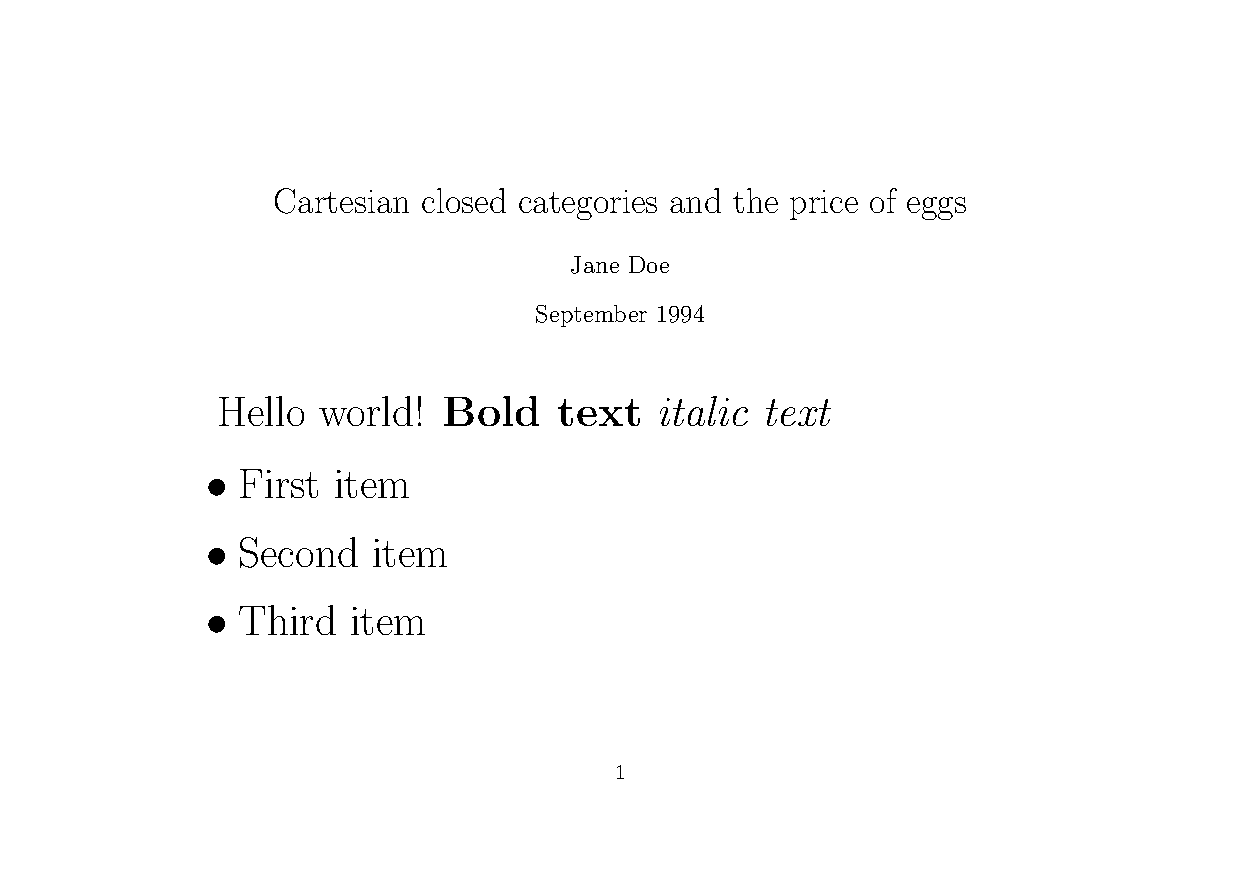
\includegraphics[width=0.45\textwidth, frame]{figures/text}
  \end{multicols}
\end{frame}

\begin{frame}
  \frametitle{Basic \LaTeX~elements -- Document structure}

  \vspace{0.5cm}

  \begin{multicols}{2}
    \lstinputlisting{examples/doc_structure.tex}

    \columnbreak

    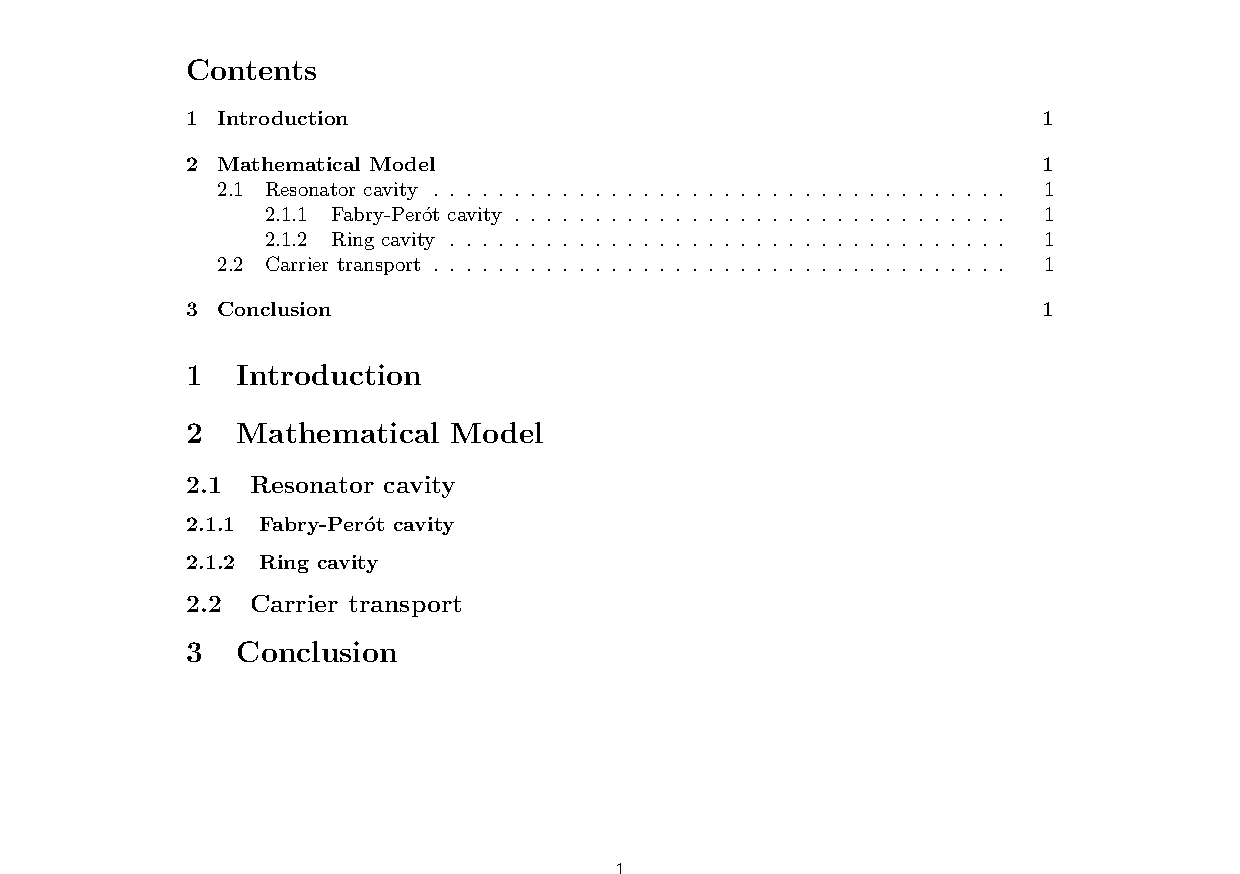
\includegraphics[width=0.45\textwidth, frame]{figures/doc_structure}
  \end{multicols}
\end{frame}

\begin{frame}
  \frametitle{Basic \LaTeX~elements -- Figures and tables}

  \vspace{0.5cm}

  \begin{multicols}{2}
    \lstinputlisting{examples/figure.tex}

    \columnbreak

    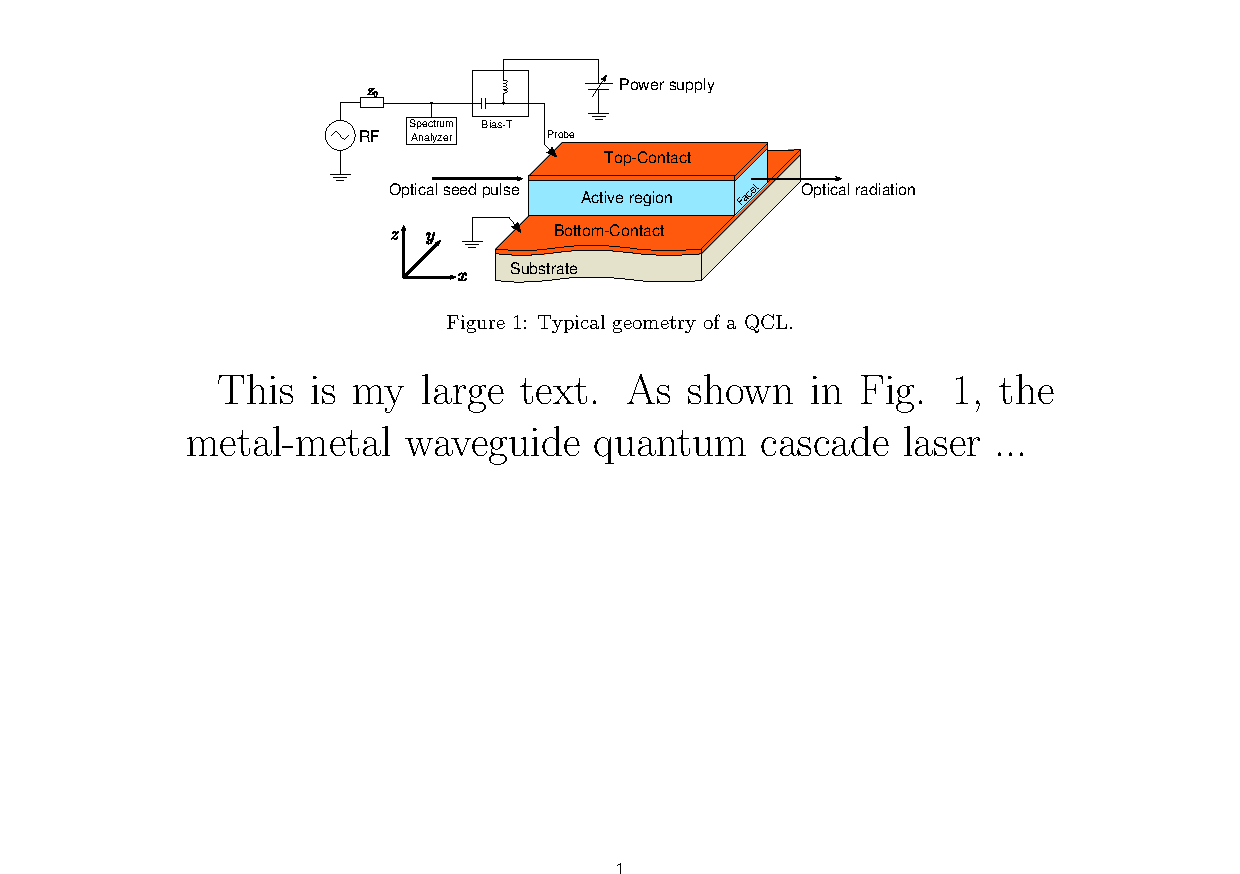
\includegraphics[width=0.45\textwidth, frame]{figures/figure}
  \end{multicols}
\end{frame}

\begin{frame}
  \frametitle{Basic \LaTeX~elements -- Mathematical equations}

  \vspace{0.5cm}

  \begin{multicols}{2}
    \lstinputlisting{examples/equations.tex}

    \columnbreak

    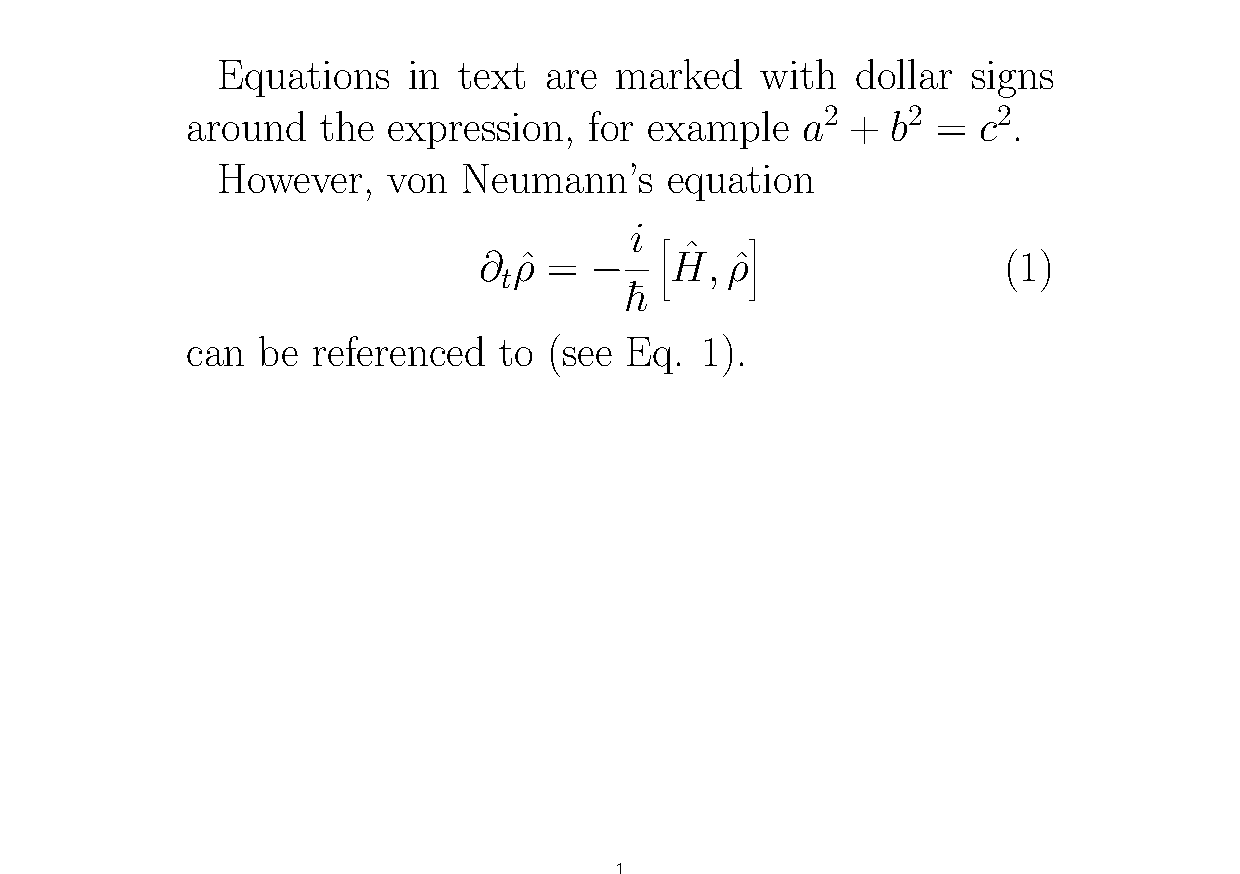
\includegraphics[width=0.45\textwidth, frame]{figures/equations}
  \end{multicols}
\end{frame}

\begin{frame}
\frametitle{How to get started}

Installation
\begin{PraesentationAufzaehlung}
\item Windows
  \begin{itemize}
  \item MIKTeX is a \TeX~distribution, TeXnicCenter and Texmaker are editors
  \item \url{http://www.howtotex.com/howto/installing-latex-on-windows/}
  \end{itemize}
\item Mac OS X
  \begin{itemize}
  \item For example, there is MacTeX and Texmaker
  \item \url{http://www.howtotex.com/howto/installing-latex-on-mac-os-x/}
  \end{itemize}
\item Linux
  \begin{itemize}
    \item Multitude of distributions and flavors
    \item For Debian one can install \texttt{texlive} and \texttt{texmaker} via the packet manager
    \item Sometimes it makes sense to download and install TeXLive directly
  \end{itemize}
\end{PraesentationAufzaehlung}
Tutorials
\begin{PraesentationAufzaehlung}
\item Enter ``latex tutorial'' into the search engine of your choice
\item Search for issues and error messages (the links to \url{http://stackoverflow.com} are generally a good choice)
\end{PraesentationAufzaehlung}
\end{frame}

\begin{frame}
  \frametitle{Build automation and tools}
  Build automation
  \begin{PraesentationAufzaehlung}
  \item For \LaTeX: Does your editor provide it? \texttt{latexmk} command available?
  \item For \LaTeX~or complete project with extra tools: \texttt{make}
  \end{PraesentationAufzaehlung}

  Tools
  \begin{PraesentationAufzaehlung}
  \item Create plots of data
    \begin{itemize}
    \item gnuplot (open-source)
    \item MATLAB (proprietary)
    \end{itemize}
  \item Vector graphics
    \begin{itemize}
    \item inkscape (open-source)
    \item tikz/pgf (\LaTeX~package)
    \end{itemize}
  \end{PraesentationAufzaehlung}

  \begin{textblock*}{0.6\paperwidth}[1,1](\textwidth + \PraesentationSeitenrand, \textheight - \PraesentationSeitenrand)%
    \begin{figure}
      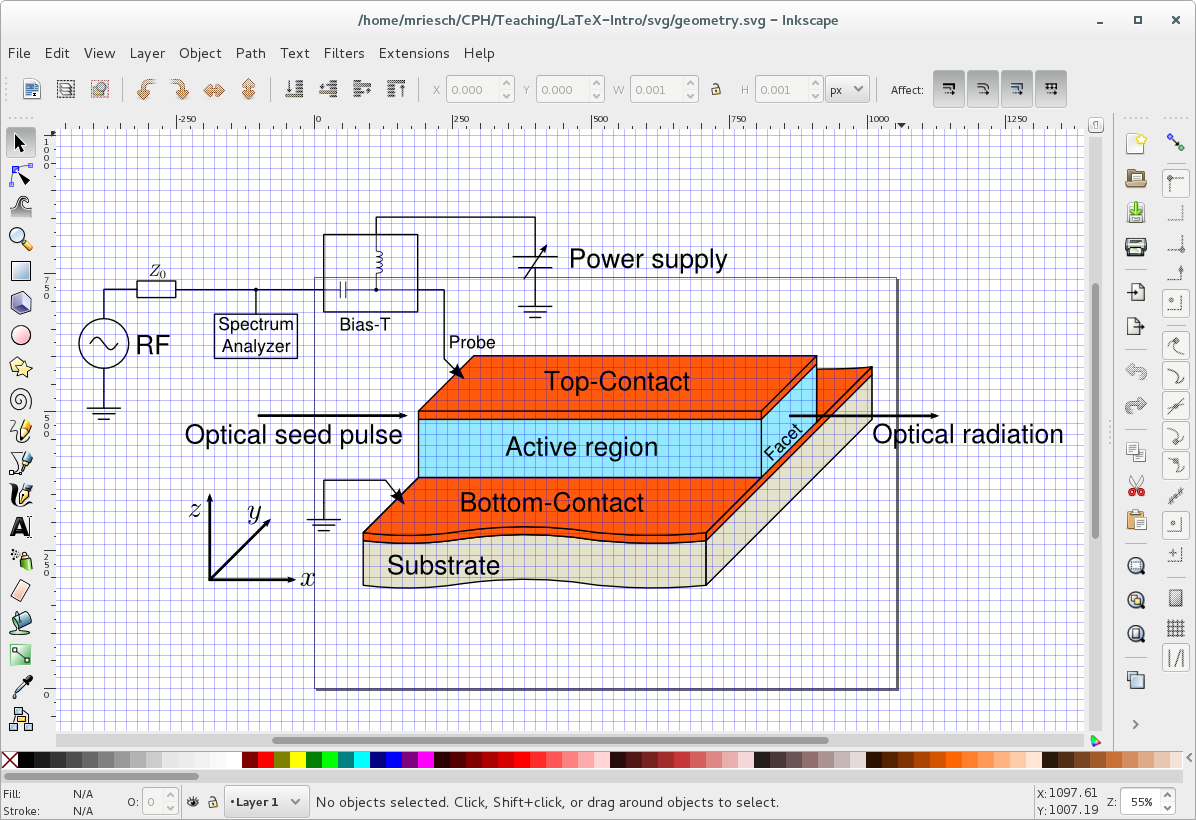
\includegraphics[width=0.5\paperwidth]{figures/inkscape}
      \caption{The inkscape vector graphics editor.}
    \end{figure}
  \end{textblock*}

\end{frame}

\begin{frame}
  \frametitle{Version control with git}

  Is version control really necessary?
  \begin{PraesentationAufzaehlung}
  \item Do you want to make backups?
  \item Are you working in a group?
  \item Do you want to keep track of the changes you and your co-workers made?
  \end{PraesentationAufzaehlung}

  The git version control system
  \begin{PraesentationAufzaehlung}
  \item open-source, distributed, scales from small projects to e.g.\ the Linux Kernel
  \item Private repositories available \@\url{bitbucket.com}, public repositories \@\url{github.com}
  \item Steep learning curve, but mostly a small subset of commands will do for you
  \end{PraesentationAufzaehlung}

\end{frame}

\begin{frame}
  \frametitle{TUM templates and style}

  TUM Corporate Design (\url{tum.de/cd}) provides \LaTeX~templates for
  \begin{PraesentationAufzaehlung}
  \item Presentation slides (based on \texttt{beamer})
  \item Theses (based on \texttt{scrbook})
  \item Letters and office papers
  \end{PraesentationAufzaehlung}

  Additionally, there is a design guide (see TUM CD homepage).

  There is work in progress. We will keep you posted and provide you with templates for your theses and presentation slides.
\end{frame}

\begin{frame}
\frametitle{Thank you for your attention!}

Contact me (michael.riesch@tum.de) if you have questions about the templates.

  \begin{textblock*}{0.65\paperwidth}[1,1](\textwidth + \PraesentationSeitenrand, \textheight - \PraesentationSeitenrand)%
    \begin{figure}
      
\includegraphics[width=0.6\paperwidth]{figures/latex-project-logo}
    \end{figure}
  \end{textblock*}


\end{frame}

\end{document}
